\documentclass[11pt,a4paper]{report}
\usepackage[textwidth=37em,vmargin=30mm]{geometry}
\usepackage{calc,xunicode,amsmath,amssymb,paralist,enumitem,tabu,booktabs,datetime2,xeCJK,xeCJKfntef,listings}
\usepackage{tocloft,fancyhdr,tcolorbox,xcolor,graphicx,eso-pic,xltxtra,xelatexemoji}

\newcommand{\envyear}[0]{2024}
\newcommand{\envdatestr}[0]{2024-11-14}
\newcommand{\envfinaldir}[0]{webdb/2024/20241114/final}

\usepackage[hidelinks]{hyperref}
\hypersetup{
    colorlinks=false,
    pdfpagemode=FullScreen,
    pdftitle={Web Digest - \envdatestr}
}

\setlength{\cftbeforechapskip}{10pt}
\renewcommand{\cftchapfont}{\rmfamily\bfseries\large\raggedright}
\setlength{\cftbeforesecskip}{2pt}
\renewcommand{\cftsecfont}{\sffamily\small\raggedright}

\setdefaultleftmargin{2em}{2em}{1em}{1em}{1em}{1em}

\usepackage{xeCJK,xeCJKfntef}
\xeCJKsetup{PunctStyle=plain,RubberPunctSkip=false,CJKglue=\strut\hskip 0pt plus 0.1em minus 0.05em,CJKecglue=\strut\hskip 0.22em plus 0.2em}
\XeTeXlinebreaklocale "zh"
\XeTeXlinebreakskip = 0pt


\setmainfont{Brygada 1918}
\setromanfont{Brygada 1918}
\setsansfont{IBM Plex Sans}
\setmonofont{JetBrains Mono NL}
\setCJKmainfont{Noto Serif CJK SC}
\setCJKromanfont{Noto Serif CJK SC}
\setCJKsansfont{Noto Sans CJK SC}
\setCJKmonofont{Noto Sans CJK SC}

\setlength{\parindent}{0pt}
\setlength{\parskip}{8pt}
\linespread{1.15}

\lstset{
	basicstyle=\ttfamily\footnotesize,
	numbersep=5pt,
	backgroundcolor=\color{black!5},
	showspaces=false,
	showstringspaces=false,
	showtabs=false,
	tabsize=2,
	captionpos=b,
	breaklines=true,
	breakatwhitespace=true,
	breakautoindent=true,
	linewidth=\textwidth
}






\newcommand{\coverpic}[2]{
    % argv: itemurl, authorname
    Cover photo by #2~~(\href{#1}{#1})
}
\newcommand{\makeheader}[0]{
    \begin{titlepage}
        % \newgeometry{hmargin=15mm,tmargin=21mm,bmargin=12mm}
        \begin{center}
            
            \rmfamily\scshape
            \fontspec{BaskervilleF}
            \fontspec{Old Standard}
            \fontsize{59pt}{70pt}\selectfont
            WEB\hfill DIGEST
            
            \vfill
            % \vskip 30pt
            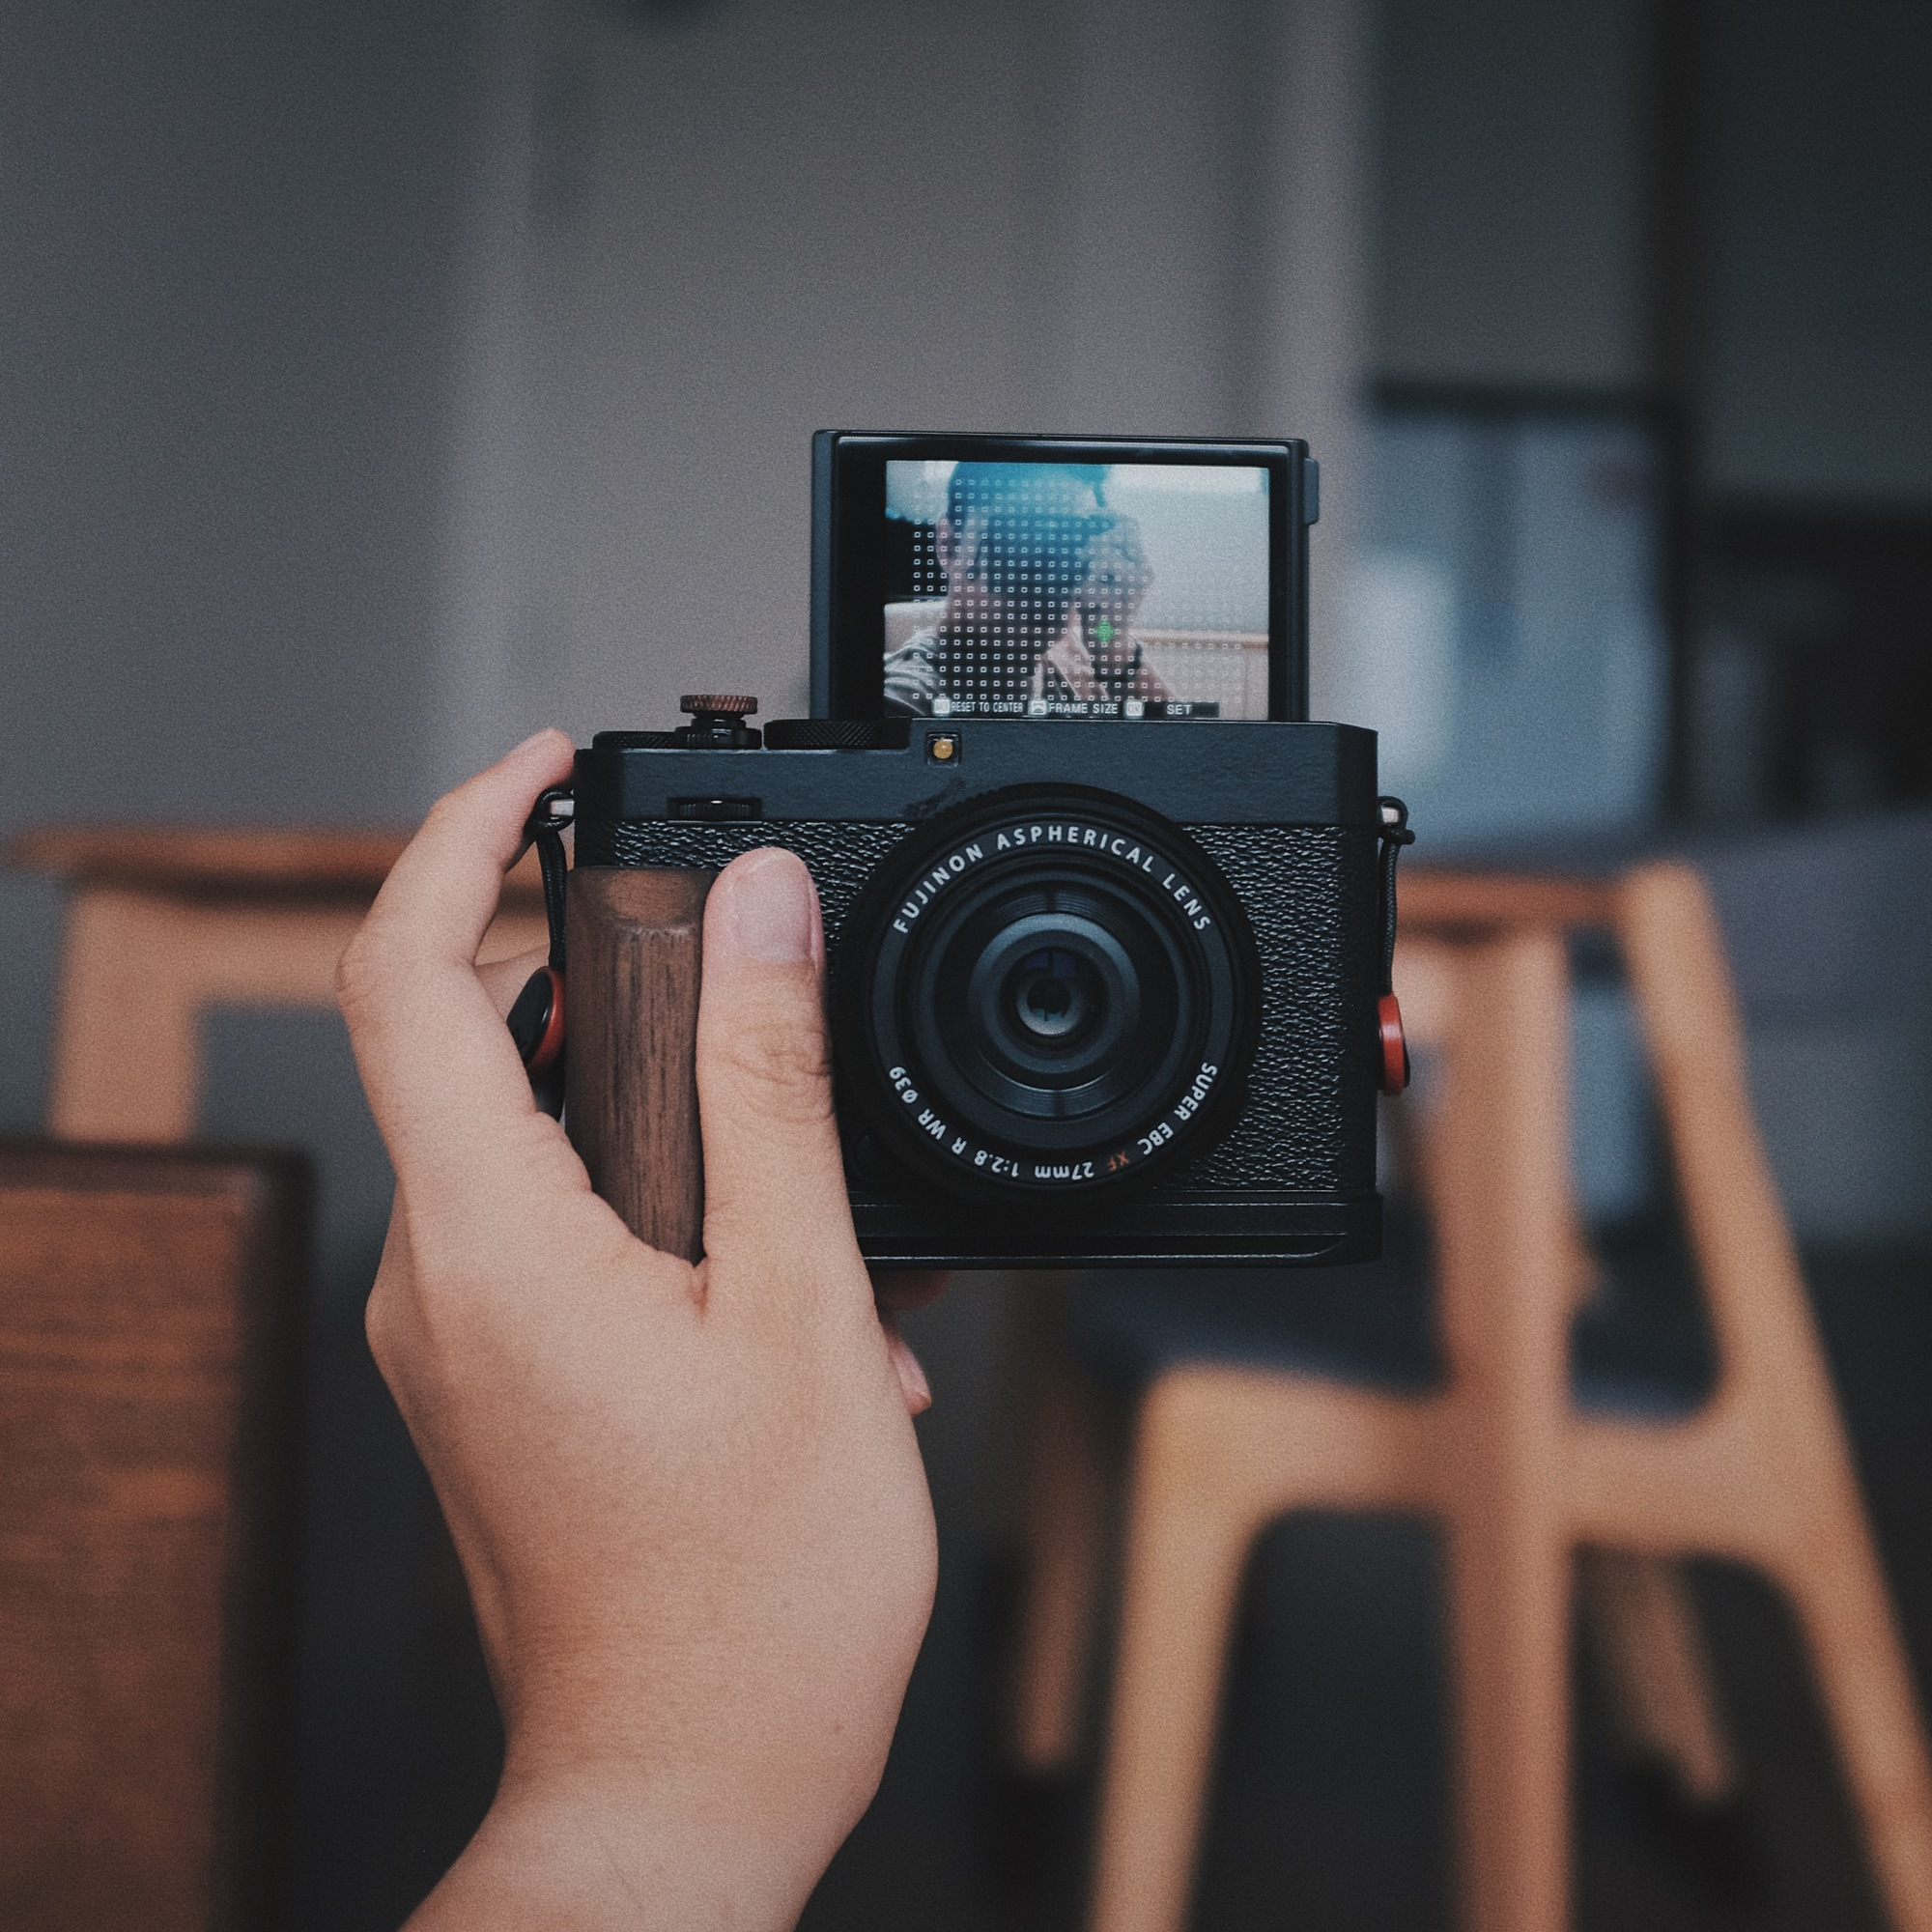
\includegraphics[width=\linewidth]{\envfinaldir/coverpic-prod.jpg}\par
            % \vskip 30pt
            \vfill

            \normalsize\rmfamily\scshape
            \copyright{} The Web Digest Project \hfill\large \envdatestr
        \end{center}
    \end{titlepage}
    % \restoregeometry
}
\newcommand{\simplehref}[1]{%
    \textcolor{blue!80!green}{\href{#1}{#1}}%
}
\renewcommand{\contentsname}{\center\Huge\sffamily\bfseries Contents\par\vskip 20pt}
\newcounter{ipartcounter}
\setcounter{ipartcounter}{0}
\newcommand{\ipart}[1]{
    % \vskip 20pt
    \clearpage
    \stepcounter{ipartcounter}
    \phantomsection
    \addcontentsline{toc}{chapter}{#1}
    % \begin{center}
    %     \Huge
    %     \sffamily\bfseries
    %     #1
    % \end{center}
    % \vskip 20pt plus 7pt
}
\newcounter{ichaptercounter}
\setcounter{ichaptercounter}{0}
\newcommand{\ichapter}[1]{
    % \vskip 20pt
    \clearpage
    \stepcounter{ichaptercounter}
    \phantomsection
    \addcontentsline{toc}{section}{\numberline{\arabic{ichaptercounter}}#1}
    \begin{center}
        \Huge
        \sffamily\bfseries
        #1
    \end{center}
    \vskip 20pt plus 7pt
}
\newcommand{\entrytitlefont}[1]{\subsection*{\raggedright\Large\sffamily\bfseries#1}}
\newcommand{\entryitemGeneric}[2]{
    % argv: title, url
    \parbox{\linewidth}{
        \entrytitlefont{#1}\par\vskip 5pt
        \footnotesize\ttfamily\mdseries
        \simplehref{#2}
    }\vskip 11pt plus 11pt minus 1pt
}
\newcommand{\entryitemGithub}[3]{
    % argv: title, url, desc
    \parbox{\linewidth}{
        \entrytitlefont{#1}\par\vskip 5pt
        \footnotesize\ttfamily\mdseries
        \simplehref{#2}\par\vskip 5pt
        \small\rmfamily\mdseries#3
    }\vskip 11pt plus 11pt minus 1pt
}
\newcommand{\entryitemAp}[3]{
    % argv: title, url, desc
    \parbox{\linewidth}{
        \entrytitlefont{#1}\par\vskip 5pt
        \footnotesize\ttfamily\mdseries
        \simplehref{#2}\par\vskip 5pt
        \small\rmfamily\mdseries#3
    }\vskip 11pt plus 11pt minus 1pt
}
\newcommand{\entryitemHackernews}[3]{
    % argv: title, hnurl, rawurl
    % \parbox{\linewidth}{
    %     \entrytitlefont{#1}\par\vskip 5pt
    %     \footnotesize\ttfamily\mdseries
    %     \simplehref{#3}\par
    %     \textcolor{black!50}{\href{#2}{#2}}
    % }\vskip 11pt plus 11pt minus 1pt
    \begin{minipage}{\linewidth}
            \entrytitlefont{#1}\par\vskip 5pt
            \footnotesize\ttfamily\mdseries
            \simplehref{#3}\par
            \textcolor{black!50}{\href{#2}{#2}}
    \end{minipage}\par\vskip 11pt plus 11pt minus 1pt
}







\begin{document}

\makeheader

\tableofcontents\clearpage




\ipart{Developers}
\ichapter{Hacker News}
\entryitemTwoLinks{Amazon Makes It Harder for Disabled Employees to Work from Home}{https://news.ycombinator.com/item?id=42130079}{https://www.bloomberg.com/news/articles/2024-11-13/amazon-makes-it-harder-for-disabled-employees-to-work-from-home}

\entryitemTwoLinks{Why the Guardian is no longer posting on X}{https://news.ycombinator.com/item?id=42129924}{https://www.theguardian.com/media/2024/nov/13/why-the-guardian-is-no-longer-posting-on-x}

\entryitemTwoLinks{A Student's Guide to Writing with ChatGPT}{https://news.ycombinator.com/item?id=42129064}{https://openai.com/chatgpt/use-cases/student-writing-guide/}

\entryitemTwoLinks{Wonder is acquiring Grubhub}{https://news.ycombinator.com/item?id=42128935}{https://about.grubhub.com/news/wonder-announces-acquisition-of-grubhub/}

\entryitemTwoLinks{My company has banned the use of Jetbrains IDEs internally}{https://news.ycombinator.com/item?id=42128866}{https://old.reddit.com/r/ExperiencedDevs/comments/1gqj7qa/my\_company\_has\_banned\_the\_use\_of\_jetbrains\_ides/}

\entryitemTwoLinks{The Impact of Jungle Music in 90s Video Game Development}{https://news.ycombinator.com/item?id=42128717}{https://pikuma.com/blog/jungle-music-video-game-drum-bass}

\entryitemTwoLinks{MIT engineers make converting CO2 into useful products more practical}{https://news.ycombinator.com/item?id=42126984}{https://news.mit.edu/2024/mit-engineers-make-converting-co2-into-products-more-practical-1113}

\entryitemTwoLinks{Show HN: Bluetooth USB Peripheral Relay – Bridge Bluetooth Devices to USB}{https://news.ycombinator.com/item?id=42125863}{https://github.com/bahaaador/bluetooth-usb-peripheral-relay}

\entryitemTwoLinks{An unearthly spectacle – The untold story of the biggest nuclear bomb (2021)}{https://news.ycombinator.com/item?id=42125085}{https://thebulletin.org/2021/11/the-untold-story-of-the-worlds-biggest-nuclear-bomb/}

\entryitemTwoLinks{U.S. Sets Targets to Triple Nuclear Energy Capacity by 2050}{https://news.ycombinator.com/item?id=42123762}{https://www.energy.gov/ne/articles/us-sets-targets-triple-nuclear-energy-capacity-2050}

\entryitemTwoLinks{Docker Compose Isn't Enough}{https://news.ycombinator.com/item?id=42122690}{https://blog.tealok.tech/post/docker-compose-isnt-enough/}

\entryitemTwoLinks{No GPS required: our app can now locate underground trains}{https://news.ycombinator.com/item?id=42122085}{https://blog.transitapp.com/go-underground/}

\entryitemTwoLinks{Spirit Airlines is filing for bankruptcy}{https://news.ycombinator.com/item?id=42121791}{https://www.wsj.com/business/airlines/spirit-airlines-moves-toward-bankruptcy-filing-after-frontier-drops-merger-bid-5d492e80}

\entryitemTwoLinks{Manjaro is experimenting with **opt-out telemetry}{https://news.ycombinator.com/item?id=42121548}{https://discuss.privacyguides.net/t/manjaro-is-experimenting-with-opt-out-telemetry/22305}

\entryitemTwoLinks{AI Hype Is Cooling – New survey}{https://news.ycombinator.com/item?id=42120331}{https://slack.com/blog/news/the-fall-2024-workforce-index-shows-ai-hype-is-cooling?nojsmode=1}

\entryitemTwoLinks{M4 Mac mini's efficiency}{https://news.ycombinator.com/item?id=42120311}{https://www.jeffgeerling.com/blog/2024/m4-mac-minis-efficiency-incredible}

\entryitemTwoLinks{Unusual Raku Features}{https://news.ycombinator.com/item?id=42120090}{https://buttondown.com/hillelwayne/archive/five-unusual-raku-features/}

\entryitemTwoLinks{Spanish police arrest ex-fraud chief after €20M found in walls of his house}{https://news.ycombinator.com/item?id=42119575}{https://www.theguardian.com/world/2024/nov/12/spanish-police-arrest-ex-fraud-chief-after-20m-found-in-walls-of-his-house}

\entryitemTwoLinks{Russian family lived alone in the Siberian wilderness for 40 years (2013)}{https://news.ycombinator.com/item?id=42119219}{https://www.smithsonianmag.com/history/this-russian-family-lived-alone-in-the-siberian-wilderness-for-40-years-unaware-of-world-war-ii-or-the-moon-landing-7354256/}

\entryitemTwoLinks{Show HN: Jelly – A simpler shared inbox for small teams}{https://news.ycombinator.com/item?id=42119042}{https://letsjelly.com/}\ichapter{Phoronix}
\entryitemGeneric{\hskip 0pt{}Mesa 24.3-rc2 Brings Fixes For Intel \& NVK Drivers}{https://www.phoronix.com/news/Mesa-24.3-rc2}

\entryitemGeneric{\hskip 0pt{}Apple M4 Mac Mini With macOS vs. Intel / AMD With Ubuntu Linux Performance}{https://www.phoronix.com/review/apple-m4-intel-amd-linux}

\entryitemGeneric{\hskip 0pt{}Ubuntu 25.04 To Further Enhance Its Installer, Aims For Linux 6.14 Kernel}{https://www.phoronix.com/news/Ubuntu-25.04-Early-Plans}

\entryitemGeneric{\hskip 0pt{}RISC-V Motherboard For Framework 13 Pricing Starts At \$368 In Early Access, \$928 For Laptop}{https://www.phoronix.com/news/RISC-V-Framework-Early-Access}

\entryitemGeneric{\hskip 0pt{}GNU C Library Merges Support for getrandom vDSO}{https://www.phoronix.com/news/glibc-getrandom-vDSO-Merged}

\entryitemGeneric{\hskip 0pt{}Intel's Zswap IAA Compress Batching Work Is Very Interesting For Linux Performance}{https://www.phoronix.com/news/Intel-Zswap-IAA-Compress-Batch}

\entryitemGeneric{\hskip 0pt{}NVIDIA MLX5 Introducing Data Direct Placement "DDP" In Linux 6.13 For Boosting Bandwidth}{https://www.phoronix.com/news/NVIDIA-MLX5-DDP-Linux}

\entryitemGeneric{\hskip 0pt{}Uncached Buffered IO Is Performing Great, Working Now On Btrfs / EXT4 / XFS}{https://www.phoronix.com/news/Uncached-Buffered-IO-2024}

\entryitemGeneric{\hskip 0pt{}AMD Continues Backing AlmaLinux For Community Enterprise Linux OS}{https://www.phoronix.com/news/AMD-AlmaLinux-2024}


\ipart{Developers~~~~(zh-Hans)}
\ichapter{Solidot}
\entryitemGeneric{\hskip 0pt{}AI大神李继刚空降PEC大会,解锁你的专属}{https://www.solidot.org/story?sid=79764}

\entryitemGeneric{\hskip 0pt{}中国品牌电视机占日本五成市场份额}{https://www.solidot.org/story?sid=79763}

\entryitemGeneric{\hskip 0pt{}额外一年的教育对大脑结构变化没有产生长期影响}{https://www.solidot.org/story?sid=79762}

\entryitemGeneric{\hskip 0pt{}Red Hat 收购 Neural Magic,将开源其技术 }{https://www.solidot.org/story?sid=79761}

\entryitemGeneric{\hskip 0pt{}木星质量双星如何形成}{https://www.solidot.org/story?sid=79760}

\entryitemGeneric{\hskip 0pt{}中国在珠海航展展示了新隐形战斗机 }{https://www.solidot.org/story?sid=79759}

\entryitemGeneric{\hskip 0pt{}因空气污染相关疾病剧增巴基斯坦临时限制户外活动}{https://www.solidot.org/story?sid=79758}

\entryitemGeneric{\hskip 0pt{}微软计划年底前移除 Windows 11 的 Mail 和 Calendar 应用}{https://www.solidot.org/story?sid=79757}

\entryitemGeneric{\hskip 0pt{}更多 X 用户逃到 Bluesky}{https://www.solidot.org/story?sid=79756}

\entryitemGeneric{\hskip 0pt{}俄罗斯的可重复使用火箭计划}{https://www.solidot.org/story?sid=79755}

\entryitemGeneric{\hskip 0pt{}Firefox 将人和隐私置于利润之上}{https://www.solidot.org/story?sid=79754}

\entryitemGeneric{\hskip 0pt{}Google 要求 Android 芯片组支持 Virtualization Framework }{https://www.solidot.org/story?sid=79753}

\entryitemGeneric{\hskip 0pt{}Ilya Sutskever 认为大模型规模已经达到平台期}{https://www.solidot.org/story?sid=79752}

\entryitemGeneric{\hskip 0pt{}双 11 购物节没有恢复往日的火热}{https://www.solidot.org/story?sid=79751}

\entryitemGeneric{\hskip 0pt{}病毒学家用其在实验室培养的病毒治疗自己的癌症}{https://www.solidot.org/story?sid=79750}

\entryitemGeneric{\hskip 0pt{}亚马逊证实员工信息泄露}{https://www.solidot.org/story?sid=79749}

\entryitemGeneric{\hskip 0pt{}FTX 起诉币安及其前 CEO 赵长鹏}{https://www.solidot.org/story?sid=79748}

\entryitemGeneric{\hskip 0pt{}披头士《Now And Then》成为首个获格莱美提名的 AI 辅助创作的歌曲}{https://www.solidot.org/story?sid=79747}

\entryitemGeneric{\hskip 0pt{}友讯证实不会修复旧型号 NAS 设备的高危漏洞}{https://www.solidot.org/story?sid=79746}

\entryitemGeneric{\hskip 0pt{}大部分中风是可以预防的}{https://www.solidot.org/story?sid=79745}\ichapter{V2EX}
\entryitemGeneric{\hskip 0pt{}[分享发现] Windows 应用商店里面的腾讯应用宝 - 初体验}{https://www.v2ex.com/t/1089362}

\entryitemGeneric{\hskip 0pt{}[问与答] 出狱半年,后续的打算}{https://www.v2ex.com/t/1089361}

\entryitemGeneric{\hskip 0pt{}[推广] 这个香水挺独特的}{https://www.v2ex.com/t/1089359}

\entryitemGeneric{\hskip 0pt{}[iPhone] ios 的钥匙链清理工具 KCleaner V2.4 已发布}{https://www.v2ex.com/t/1089358}

\entryitemGeneric{\hskip 0pt{}[生活] 回海南第三个月,冒个泡}{https://www.v2ex.com/t/1089357}

\entryitemGeneric{\hskip 0pt{}[macOS] macOS Stable Diffusion ?}{https://www.v2ex.com/t/1089356}

\entryitemGeneric{\hskip 0pt{}[macOS] macmini m4pro windowserver 占用}{https://www.v2ex.com/t/1089355}

\entryitemGeneric{\hskip 0pt{}[问与答] 带眼镜+骨传导耳机,体验好吗?}{https://www.v2ex.com/t/1089354}

\entryitemGeneric{\hskip 0pt{}[Apple] Mac mini M4 京东国补抢购经验}{https://www.v2ex.com/t/1089352}

\entryitemGeneric{\hskip 0pt{}[Windows] Windwos 中 chrome 浏览器显示由贵组织管理}{https://www.v2ex.com/t/1089351}

\entryitemGeneric{\hskip 0pt{}[Apple] 以前国区美区 app 都自动更新 不知道何时不行了}{https://www.v2ex.com/t/1089350}

\entryitemGeneric{\hskip 0pt{}[推广] 我来给朋友的可视化低代码平民级 RPA 和指纹浏览器项目拉个风投!}{https://www.v2ex.com/t/1089348}

\entryitemGeneric{\hskip 0pt{}[程序员] 为什么工作后对于代码的热情下降了}{https://www.v2ex.com/t/1089347}

\entryitemGeneric{\hskip 0pt{}[Apple] 日版的 iPhone 如果不去日本,是不是目前最优的选择,另外美区 ID,美国银行卡,登陆后能买 AC 么}{https://www.v2ex.com/t/1089346}

\entryitemGeneric{\hskip 0pt{}[酷工作] Telegram 小程序 后台开发外包 工作}{https://www.v2ex.com/t/1089345}

\entryitemGeneric{\hskip 0pt{}[问与答] 为什么 chrome 和 firefox 都只在 https 下请求 zstd 编码的内容}{https://www.v2ex.com/t/1089343}

\entryitemGeneric{\hskip 0pt{}[香港] 关于过香港开户的问题}{https://www.v2ex.com/t/1089342}

\entryitemGeneric{\hskip 0pt{}[iOS] 求 IOS18 相册重复照片清理方法}{https://www.v2ex.com/t/1089341}

\entryitemGeneric{\hskip 0pt{}[macOS] EXT4 转 APFS 有什么方案么?}{https://www.v2ex.com/t/1089340}

\entryitemGeneric{\hskip 0pt{}[分享创造] 分享一个我最近做的 3D 打印资源导航网站}{https://www.v2ex.com/t/1089337}

\entryitemGeneric{\hskip 0pt{}[分享创造] 音简音乐编辑 APP 项目}{https://www.v2ex.com/t/1089336}

\entryitemGeneric{\hskip 0pt{}[南京] 各位大佬我司准备做线上+线下相亲大家有什么意见或建议}{https://www.v2ex.com/t/1089334}

\entryitemGeneric{\hskip 0pt{}[新手求助] 小区业主老是喜欢车库遛狗,狗老在我车位拉屎拉尿,求助!}{https://www.v2ex.com/t/1089333}

\entryitemGeneric{\hskip 0pt{}[YouTube] 请更新你的付款方式,以继续使用 YouTube Premium}{https://www.v2ex.com/t/1089331}

\entryitemGeneric{\hskip 0pt{}[OpenAI] WildCard 亲测可以支付 ChatGPT Plus}{https://www.v2ex.com/t/1089330}

\entryitemGeneric{\hskip 0pt{}[问与答] 中银香港的 app 一打开就闪退,说你的设备有安全风险,求助}{https://www.v2ex.com/t/1089329}

\entryitemGeneric{\hskip 0pt{}[MySQL] 铁子们,求助 docker 中 MySQL 导入数据库速度问题}{https://www.v2ex.com/t/1089328}

\entryitemGeneric{\hskip 0pt{}[Apple] 雷雳 4 充电 MBA 有电流声正常吗?}{https://www.v2ex.com/t/1089327}

\entryitemGeneric{\hskip 0pt{}[问与答] 设备太多也是烦恼😣}{https://www.v2ex.com/t/1089325}

\entryitemGeneric{\hskip 0pt{}[问与答] 存了一些音乐在阿里云盘上,今天打算下载回来,发现文件已被冻结无法下载了。有什么办法可以解冻吗}{https://www.v2ex.com/t/1089324}

\entryitemGeneric{\hskip 0pt{}[问与答] MacOS 卸载 App 怎么那么的难,完全找不着方向。}{https://www.v2ex.com/t/1089323}

\entryitemGeneric{\hskip 0pt{}[问与答] 有没有这样的 sql 分析工具, mysql 举例}{https://www.v2ex.com/t/1089322}

\entryitemGeneric{\hskip 0pt{}[问与答] 再见爱人 4 如果有这 2 个飞行嘉宾}{https://www.v2ex.com/t/1089321}

\entryitemGeneric{\hskip 0pt{}[问与答] Ubuntu22.04 容器中可以安装 Oracle19c 吗?}{https://www.v2ex.com/t/1089319}

\entryitemGeneric{\hskip 0pt{}[macOS] mac 有办法裸 mihomo 内核使用 TUN 模式吗}{https://www.v2ex.com/t/1089318}

\entryitemGeneric{\hskip 0pt{}[分享创造] 🤖 [分享贴] 我如何使用 ChatGPT-o1 和 Cursor 在一天全程完成 [ TrendX.wiki ] 的搭建,几乎 0 手写}{https://www.v2ex.com/t/1089317}

\entryitemGeneric{\hskip 0pt{}[Apple] 谁能用 M4 的 Macmini 测试下运行 Ryujinx 玩塞尔达的效果呀?}{https://www.v2ex.com/t/1089316}

\entryitemGeneric{\hskip 0pt{}[Apple] 我一直觉得 Mac mini 的电源按键没问题...直到我拿出 Magic Keyboard}{https://www.v2ex.com/t/1089315}

\entryitemGeneric{\hskip 0pt{}[问与答] 问问大伙家里电视用的是什么盒子}{https://www.v2ex.com/t/1089314}

\entryitemGeneric{\hskip 0pt{}[Pixel] 现在 pixel 一代还可以无限量传输照片吗?}{https://www.v2ex.com/t/1089313}

\entryitemGeneric{\hskip 0pt{}[iPhone] 看到有机械加工换 C 口的}{https://www.v2ex.com/t/1089312}

\entryitemGeneric{\hskip 0pt{}[问与答] 有没有性价比高的迷你主机?}{https://www.v2ex.com/t/1089310}

\entryitemGeneric{\hskip 0pt{}[北京] 今天早高峰从慧中桥到四元桥一路为何堵的死死的?}{https://www.v2ex.com/t/1089308}

\entryitemGeneric{\hskip 0pt{}[OpenAI] 一键生成精彩解说短视频(模型更新)}{https://www.v2ex.com/t/1089307}

\entryitemGeneric{\hskip 0pt{}[Apple] 授权店买苹果产品有优惠吗}{https://www.v2ex.com/t/1089305}

\entryitemGeneric{\hskip 0pt{}[杭州] 契税刚交完,怎么弄}{https://www.v2ex.com/t/1089304}

\entryitemGeneric{\hskip 0pt{}[问与答] 有必要买一台类似 Kindle 的墨水屏电子书阅读器吗}{https://www.v2ex.com/t/1089303}

\entryitemGeneric{\hskip 0pt{}[OpenAI] WildCard 疑似被脱裤导致盗刷}{https://www.v2ex.com/t/1089302}

\entryitemGeneric{\hskip 0pt{}[Apple] 作为一个文字工作者,曾以为 48G 内存只是满足我的购物欲,直到……}{https://www.v2ex.com/t/1089300}

\entryitemGeneric{\hskip 0pt{}[VMware] 大新闻! VMware Workstation Pro 商业免费}{https://www.v2ex.com/t/1089299}


\ipart{Generic News}
\ichapter{AP News}
\entryitemWithDescription{\hskip 0pt{}Prominent conservative lawyer Ted Olson, who argued Bush recount and same-sex marriage cases, dies}{https://apnews.com/article/68d5fe56bad7640cb2b325f82ae0cbc7}{}

\entryitemWithDescription{\hskip 0pt{}Spurs coach Gregg Popovich had a stroke earlier this month}{https://apnews.com/article/26fdfd84655c42536a5d90ac82f7162e}{}

\entryitemWithDescription{\hskip 0pt{}MMA star Conor McGregor says sexual assault claim is `full blown lie among many lies'}{https://apnews.com/article/7e0e014c7ee3822723349328565b406d}{}

\entryitemWithDescription{\hskip 0pt{}A wayward sea turtle wound up in the Netherlands. A rescue brought it thousands of miles back home}{https://apnews.com/article/c625e0085e3a3966d546ab51de0ece3f}{}

\entryitemWithDescription{\hskip 0pt{}Alex Jones hopes Infowars auction lets him stay on its platforms}{https://apnews.com/article/c613c8fa6276936a10d0656e4e424b8e}{}

\entryitemWithDescription{\hskip 0pt{}Massive dust storm causes a vehicle pileup on central California highway}{https://apnews.com/article/c5d17803081a98b772e102c375addaf2}{}

\entryitemWithDescription{\hskip 0pt{}Dogecoin soars as Trump announces a government efficiency group nicknamed DOGE}{https://apnews.com/article/5a6f9d61ad7c5d4fc94f567dd9ee090e}{}

\entryitemWithDescription{\hskip 0pt{}Homes of Chiefs' quarterback Mahomes and tight end Kelce were broken into last month}{https://apnews.com/article/f62b0778066f9f3bf0c196019118a42a}{}

\entryitemWithDescription{\hskip 0pt{}Bad Bunny's baseball agency punishment upheld}{https://apnews.com/article/1d7432188f11806f55e99f7f457a95cc}{}

\entryitemWithDescription{\hskip 0pt{}Wander Franco released under supervision after gun arrest in Dominican Republic}{https://apnews.com/article/4480484a86f80110394a333001ac6098}{}

\entryitemWithDescription{\hskip 0pt{}Timothy West, acclaimed British actor and lover of UK's waterways, dies aged 90}{https://apnews.com/article/24dcadb6aac00b16363033f3328fb733}{}

\entryitemWithDescription{\hskip 0pt{}GM recalling big pickups and SUVs because the rear wheels can lock up, increasing risk of a crash}{https://apnews.com/article/9d1067efee1c2713ae8633b1965bf9c9}{}

\entryitemWithDescription{\hskip 0pt{}Oregon tops Week 2 College Football Playoff rankings and Georgia drops out of the bracket}{https://apnews.com/article/fc725ce2b5fb1d7d4f29ba88beedabac}{}\ichapter{Reuters}
\entryitemWithDescription{\hskip 0pt{}Brazil's Finance Minister signals uncertainty over fiscal package announcement this week}{https://www.reuters.com/world/americas/brazils-finance-minister-signals-uncertainty-over-fiscal-package-announcement-2024-11-13/}{Brazil\textquotesingle s Finance Minister Fernando Haddad said on Wednesday he is uncertain whether there is enough time to announce a spending containment package this week, adding that it will be released once President Luiz Inacio Lula...}

\entryitemWithDescription{\hskip 0pt{}Senior aide to Argentina's Milei says Shell eying LNG investment, according to report}{https://www.reuters.com/business/energy/senior-aide-argentinas-milei-says-shell-eying-lng-investment-according-report-2024-11-13/}{The cabinet chief to Argentine President Javier Milei cited oil major Shell as a potential investor in a future liquefied natural gas (LNG) project to be run by the country\textquotesingle s state oil firm YPF , according to newspaper La...}

\entryitemWithDescription{\hskip 0pt{}Exclusive: Saudi Arabia prioritizes sports for NEOM plans as costs balloon, sources say}{https://www.reuters.com/world/middle-east/saudi-arabia-prioritizes-sports-neom-plans-costs-balloon-sources-say-2024-11-13/}{Saudi Arabia has scaled back lofty ambitions for its NEOM gigaproject to prioritize completing elements essential to hosting global sporting events over the next decade as rising costs weigh, three sources told Reuters a day after the...}

\entryitemWithDescription{\hskip 0pt{}Israel wants freedom to strike Lebanon even after ceasefire, France says}{https://www.reuters.com/world/israel-wants-freedom-strike-lebanon-even-after-ceasefire-france-says-2024-11-13/}{Israeli officials are insisting on maintaining a capacity to strike Lebanon at any moment as part of conditions to secure a ceasefire with Iran-backed Hezbollah, France\textquotesingle s foreign minister said on...}

\entryitemWithDescription{\hskip 0pt{}Kyiv 'cautiously optimistic' after discussing deep strikes in Russia with US}{https://www.reuters.com/world/europe/kyiv-cautiously-optimistic-after-discussing-deep-strikes-russia-with-us-2024-11-13/}{Ukrainian Foreign Minister Andrii Sybiha said on Wednesday he was "cautiously optimistic" after discussing with U.S. Secretary of State Antony Blinken the possibility of conducting deep strikes on Russia as well as Euro-Atlantic...}

\entryitemWithDescription{\hskip 0pt{}Police detain pro-Palestinian protesters defying Amsterdam ban}{https://www.reuters.com/world/middle-east/pro-palestinian-protesters-again-defy-amsterdam-ban-2024-11-13/}{Police detained pro-Palestinian protesters rallying in central Amsterdam on Wednesday in defiance of a ban imposed after violence stemming from a football match between Ajax and Israeli club Maccabi Tel...}

\entryitemWithDescription{\hskip 0pt{}Entire generation in Gaza would lose education if UNRWA collapses, says UN}{https://www.reuters.com/world/middle-east/entire-generation-gaza-would-lose-education-if-unrwa-collapses-says-un-2024-11-13/}{An entire generation of Palestinians in the Gaza Strip would "be denied the right to education" if the United Nations Palestinian relief agency UNRWA collapses in the enclave under new Israeli legislation, the head of UNRWA warned on...}

\entryitemWithDescription{\hskip 0pt{}Exclusive: European powers pushing for resolution against Iran at IAEA, diplomats say}{https://www.reuters.com/world/european-powers-pushing-resolution-against-iran-iaea-diplomats-say-2024-11-13/}{The resolution would task the IAEA with issuing a "comprehensive report" on Iran\textquotesingle s nuclear activities, which would put further focus on Iran\textquotesingle s failure to explain uranium traces found at undeclared...}

\entryitemWithDescription{\hskip 0pt{}'One-of-a-kind' skull fossil from Brazil reveals bird brain evolution}{https://www.reuters.com/science/one-of-a-kind-skull-fossil-brazil-reveals-bird-brain-evolution-2024-11-13/}{The brains of today\textquotesingle s birds facilitate a level of cognitive prowess and behavioral complexity rivaled only by mammals. But how the avian brain evolved over many millions of years from an ancestral dinosaurian form has long...}

\entryitemWithDescription{\hskip 0pt{}UN nuclear watchdog chief Grossi arrives in Iran for talks}{https://www.reuters.com/world/un-nuclear-watchdog-chief-grossi-arrives-iran-talks-2024-11-13/}{U.N. atomic watchdog chief Rafael Grossi arrived in Iran for talks on Wednesday, Iranian state media reported, a day after he appealed to Iran\textquotesingle s leadership to take steps to resolve longstanding issues with his agency over...}

\entryitemWithDescription{\hskip 0pt{}France tightens security for Israel soccer match after clashes in Amsterdam}{https://www.reuters.com/world/europe/france-tightens-security-israel-soccer-match-after-clashes-amsterdam-2024-11-13/}{French authorities have stepped up security in Paris ahead of a France-Israel soccer match on Thursday, hoping to avoid a repeat of violent clashes between locals and Israeli soccer fans in Amsterdam last...}

\entryitemWithDescription{\hskip 0pt{}Israel questions ICC judge's impartiality in Netanyahu arrest case}{https://www.reuters.com/world/middle-east/israel-questions-icc-judges-impartiality-netanyahu-arrest-case-2024-11-13/}{Israel has questioned the impartiality of an International Criminal Court judge appointed to a panel deciding whether an arrest warrant should be issued for Israeli Prime Minister Benjamin...}

\entryitemWithDescription{\hskip 0pt{}Spaniards brace for fresh storms two weeks after deadly Valencia floods}{https://www.reuters.com/world/europe/spaniards-brace-fresh-storms-two-weeks-after-deadly-valencia-floods-2024-11-13/}{Spaniards braced for further heavy rain and storms on Wednesday, just two weeks after rain and flash floods prompted rivers to overflow in Valencia and other parts of Spain killing more than 200 people and destroying homes and...}






\clearpage
\leavevmode\vfill
\footnotesize

Copyright \copyright{} 2023-2024 Neruthes and other contributors.

This document is published with CC BY-NC-ND 4.0 license.

The entries listed in this newsletter may be copyrighted by their respective creators.

This newsletter is generated by the Web Digest project.

The newsletters are also delivered via Telegram channel \CJKunderline{\href{https://t.me/webdigestchannel}{https://t.me/webdigestchannel}}.\\
RSS feed is available at \CJKunderline{\href{https://webdigest.pages.dev/rss.xml}{https://webdigest.pages.dev/rss.xml}}.

This newsletter is available in PDF at
\CJKunderline{\href{https://webdigest.pages.dev/}{https://webdigest.pages.dev/}}.

The source code being used to generate this newsletter is available at\\
\CJKunderline{\href{https://github.com/neruthes/webdigest}{https://github.com/neruthes/webdigest}}.

This newsletter is also available in
\CJKunderline{\href{http://webdigest.pages.dev/readhtml/\envyear/WebDigest-20241114.html}{HTML}} and
\CJKunderline{\href{https://github.com/neruthes/webdigest/blob/master/markdown/\envyear/WebDigest-20241114.md}{Markdown}}.


\coverpic{https://unsplash.com/photos/a-person-standing-in-the-middle-of-a-forest-at-night-3LtYPz\_3T1Y}{Annie Spratt}


\end{document}
